% =============================================================================
% UNCASE: Privacy-Safe Synthetic Conversational Data for Regulated Industries
% Academic Whitepaper — NeurIPS/JMLR-style formatting
% March 2026
% =============================================================================
\documentclass[11pt,letterpaper]{article}

% ── Geometry (JMLR / NeurIPS single-column style) ──────────────────────────
\usepackage[
  top=1in,
  bottom=1in,
  left=1in,
  right=1in,
]{geometry}

% ── Typography: Computer Modern (the classic Knuth LaTeX font) ─────────────
\usepackage[T1]{fontenc}
\usepackage[utf8]{inputenc}
\usepackage{lmodern}            % Latin Modern — scalable Computer Modern (Knuth)
\usepackage{microtype}          % Microtypographic enhancements
\usepackage{setspace}
\setstretch{1.08}               % Slight stretch for readability

% ── Mathematics (AMS suite — standard in scientific publications) ──────────
\usepackage{amsmath}
\usepackage{amssymb}
\usepackage{amsthm}
\newtheorem{definition}{Definition}
\newtheorem{proposition}{Proposition}

% ── Graphics & Figures ─────────────────────────────────────────────────────
\usepackage{graphicx}
\usepackage{float}
\usepackage{tikz}
\usetikzlibrary{
  shapes.geometric, arrows.meta, positioning, calc, fit,
  backgrounds, decorations.pathreplacing, patterns
}

% ── Tables (academic style) ────────────────────────────────────────────────
\usepackage{booktabs}           % Professional table rules
\usepackage{tabularx}
\usepackage{multirow}
\usepackage{array}
\usepackage{threeparttable}     % Table footnotes (standard in journals)
\newcolumntype{L}[1]{>{\raggedright\arraybackslash}p{#1}}
\newcolumntype{C}[1]{>{\centering\arraybackslash}p{#1}}
\newcolumntype{R}[1]{>{\raggedleft\arraybackslash}p{#1}}

% ── Captions (academic style) ──────────────────────────────────────────────
\usepackage[
  font=small,
  labelfont=bf,
  labelsep=period,
  justification=centering,
]{caption}
\usepackage{subcaption}

% ── Code Listings ──────────────────────────────────────────────────────────
\usepackage{listings}
\lstset{
  basicstyle=\ttfamily\small,
  breaklines=true,
  frame=tb,
  framerule=0.4pt,
  xleftmargin=1.5em,
  xrightmargin=0.5em,
  aboveskip=0.8em,
  belowskip=0.8em,
  tabsize=2,
  showstringspaces=false,
  keywordstyle=\bfseries,
  commentstyle=\itshape\color{gray},
  numbers=left,
  numberstyle=\tiny\color{gray},
  numbersep=8pt,
}

% ── Algorithms ─────────────────────────────────────────────────────────────
\usepackage[ruled,vlined,linesnumbered]{algorithm2e}
\SetAlCapSkip{0.5em}

% ── Bibliography (natbib — standard in ML/AI venues) ──────────────────────
\usepackage[numbers,sort&compress]{natbib}

% ── Hyperlinks (subtle, academic style) ────────────────────────────────────
\usepackage[
  colorlinks=true,
  linkcolor=black,
  citecolor=blue!60!black,
  urlcolor=blue!60!black,
  bookmarks=true,
  bookmarksnumbered=true,
  pdfauthor={UNCASE Team},
  pdftitle={UNCASE: Privacy-Safe Synthetic Conversational Data for Regulated Industries},
]{hyperref}

% ── Cross-references (must load AFTER hyperref) ──────────────────────────
\usepackage[nameinlink,capitalize]{cleveref}

% ── Headers & Footers (clean academic style) ──────────────────────────────
\usepackage{fancyhdr}
\pagestyle{fancy}
\fancyhf{}
\fancyhead[L]{\small\textit{UNCASE: Privacy-Safe Synthetic Conversational Data}}
\fancyhead[R]{\small\thepage}
\renewcommand{\headrulewidth}{0.4pt}
\renewcommand{\footrulewidth}{0pt}

% ── Author block (journal style) ──────────────────────────────────────────
\usepackage{authblk}

% ── Enumerations ──────────────────────────────────────────────────────────
\usepackage{enumitem}
\setlist[itemize]{nosep, leftmargin=1.5em}
\setlist[enumerate]{nosep, leftmargin=1.5em}

% ── Custom commands ───────────────────────────────────────────────────────
\newcommand{\scsf}{\textsc{scsf}}
\newcommand{\metric}[1]{\texttt{#1}}
\newcommand{\layer}[1]{\textbf{Layer~#1}}
\newcommand{\ie}{i.e.\@\xspace}
\newcommand{\eg}{e.g.\@\xspace}
\newcommand{\etal}{\textit{et~al.}\@\xspace}
\usepackage{xspace}


% =============================================================================
% DOCUMENT
% =============================================================================
\begin{document}

% ── Title Block ───────────────────────────────────────────────────────────
\title{%
  \textbf{UNCASE: Privacy-Safe Synthetic Conversational Data\\
  for Fine-Tuning LLMs in Regulated Industries}%
}

\author[1]{Mariano Morales}
\author[1]{UNCASE Team}
\affil[1]{UNCASE AI \quad \texttt{https://uncase.md}}

\date{%
  Technical Whitepaper --- Version 2.0\\[0.3em]
  March 2026%
}

\maketitle
\thispagestyle{fancy}

% ── Abstract ──────────────────────────────────────────────────────────────
\begin{abstract}
Fine-tuning large language models (LLMs) for regulated industries---healthcare,
finance, legal, manufacturing---requires domain-specific conversational training
data that is both \emph{high-quality} and \emph{free of personally identifiable
information} (PII). We present \textbf{UNCASE} (Unbiased Neutral Convention for
Agnostic Seed Engineering), an open-source framework that implements the
\emph{Synthetic Conversation Seed Framework} (SCSF): a five-layer pipeline that
(1)~strips PII from real conversations to produce anonymized structural
blueprints called \emph{seeds}, (2)~generates thousands of synthetic
conversations guided by these seeds, (3)~evaluates quality across nine
metrics---including LLM-as-Judge semantic fidelity and embedding drift---with
hard rejection thresholds, and (4)~exports certified training data in eleven
fine-tuning formats with full tool-call support. The system includes five
compliance profiles (HIPAA, GDPR, SOX, LFPDPPP, EU~AI~Act), an adversarial
input shield, 150 curated domain seeds, 30 industry-specific tools, and
enterprise infrastructure with 106 REST API endpoints, JWT authentication, audit
logging, and observability. UNCASE is designed so that real data never reaches
the generation or training stages, providing privacy guarantees by architecture
rather than by post-hoc anonymization. We describe the framework design, quality
assurance methodology, compliance mechanisms, and deployment options.
\end{abstract}

\vspace{0.5em}
\noindent\textbf{Keywords:} synthetic data, conversational AI, fine-tuning,
LoRA, privacy, PII, regulated industries, LLM-as-Judge, differential privacy

\vspace{1em}
\hrule
\vspace{1em}


% =============================================================================
\section{Introduction}
\label{sec:introduction}
% =============================================================================

Large language models have demonstrated remarkable capabilities across
natural language tasks~\citep{brown2020gpt3,touvron2023llama,team2024gemma}.
However, deploying these models in regulated industries---healthcare, finance,
legal services, and manufacturing---requires domain-specific fine-tuning on
conversational data that reflects the terminology, decision-making patterns,
and regulatory constraints of each sector.

This creates a fundamental tension: the conversations needed for fine-tuning
contain sensitive personal data that cannot be used directly due to regulations
such as HIPAA~\citep{hipaa1996}, GDPR~\citep{gdpr2016}, SOX~\citep{sox2002},
and the EU~AI~Act~\citep{euaiact2024}. Existing approaches---manual
anonymization, rule-based scrubbing, template-based generation, and generic
LLM prompting---each fail to simultaneously preserve domain fidelity, guarantee
zero PII exposure, and provide auditable quality assurance.

We introduce \textbf{UNCASE} (Unbiased Neutral Convention for Agnostic Seed
Engineering), an open-source framework built on the \emph{Synthetic
Conversation Seed Framework} (SCSF). The key insight is that real conversations
should never be used directly for generation or training. Instead, UNCASE
extracts anonymized structural blueprints---\emph{seeds}---that capture the
conversational patterns, domain knowledge, and dialog flow without retaining
any PII. These seeds then guide the generation of entirely new synthetic
conversations that are structurally faithful to the originals but contain no
real personal data.

\paragraph{Contributions.} This paper describes the following:
\begin{enumerate}
  \item A five-layer pipeline architecture where PII removal occurs \emph{before}
    any generation or processing, providing privacy by design rather than
    post-hoc anonymization (\cref{sec:architecture}).
  \item A nine-metric quality evaluation system including two semantic
    evaluators---LLM-as-Judge rubric scoring and embedding drift
    detection---with hard rejection thresholds that prevent low-quality data
    from entering training (\cref{sec:quality}).
  \item An adversarial input protection module (PromptShield) that detects
    prompt injection, jailbreak attempts, and PII solicitation across five
    threat categories (\cref{sec:privacy}).
  \item Five frozen compliance profiles for HIPAA, GDPR, SOX, LFPDPPP, and the
    EU~AI~Act, each specifying PII categories, differential privacy budgets,
    retention policies, and quality thresholds (\cref{sec:compliance}).
  \item A production-ready implementation with 106 REST API endpoints, parallel
    pipeline orchestration, 150 curated domain seeds, 30 industry tools, 11
    export formats, and GPU deployment automation (\cref{sec:implementation}).
\end{enumerate}


% =============================================================================
\section{Related Work}
\label{sec:related}
% =============================================================================

\paragraph{Synthetic data generation.}
Approaches to synthetic data range from statistical
methods~\citep{nowok2016synthpop} and GANs~\citep{park2018dp_cgan} to
LLM-based generation~\citep{josifoski2023flows}. Most focus on tabular or
structured data; conversational data presents additional challenges in
maintaining dialog coherence, role consistency, and multi-turn factual fidelity.

\paragraph{Privacy-preserving ML.}
Differential privacy~\citep{dwork2006dp,abadi2016dpsgd} provides formal
guarantees for training data protection. Federated
learning~\citep{mcmahan2017federated} keeps data distributed. PII detection
systems such as Microsoft Presidio~\citep{presidio2023} and
spaCy~\citep{honnibal2020spacy} offer named entity recognition for
anonymization. UNCASE combines PII detection with architectural separation:
real data is transformed into abstract seeds before any LLM processing occurs.

\paragraph{LLM evaluation.}
LLM-as-Judge~\citep{zheng2024judging} uses language models to evaluate
generated text quality. ROUGE~\citep{lin2004rouge} measures surface-level
overlap. Type-token ratio (TTR) quantifies lexical
diversity~\citep{templin1957language}. UNCASE combines lexical, structural,
and semantic evaluation into a unified quality gate with mandatory thresholds.

\paragraph{Fine-tuning for domain specialization.}
LoRA~\citep{hu2022lora} and QLoRA~\citep{dettmers2023qlora} enable efficient
fine-tuning of large models. Training data quality directly impacts model
performance~\citep{zhou2024lima,chen2024alpagasus}. UNCASE provides a
complete pipeline from raw conversations to certified training data in formats
compatible with all major model architectures.


% =============================================================================
\section{The SCSF Architecture}
\label{sec:architecture}
% =============================================================================

The Synthetic Conversation Seed Framework (SCSF) is a five-layer pipeline
where each layer has a single responsibility and communicates via validated
Pydantic~v2 schemas. The architecture enforces a critical invariant:
\emph{raw conversational data never propagates beyond Layer~0}.

\begin{figure}[t]
\centering
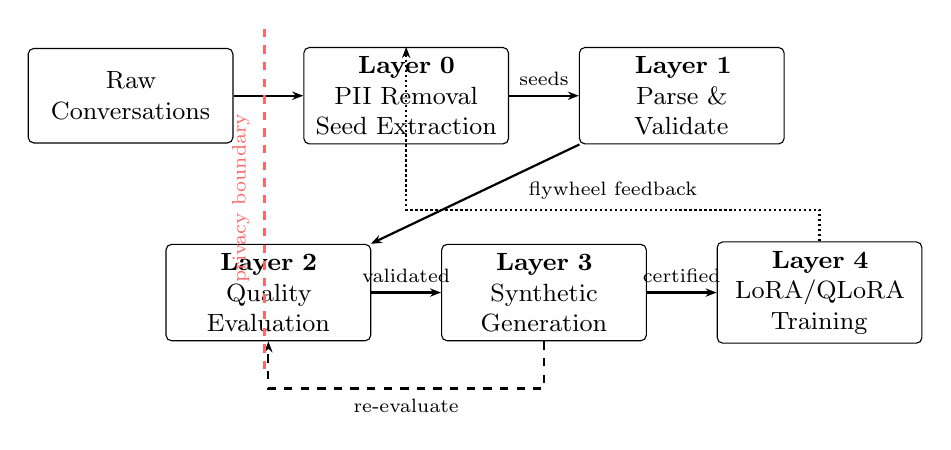
\begin{tikzpicture}[
  box/.style={draw, rounded corners=2pt, minimum width=2.6cm, minimum height=1.2cm,
    text width=2.3cm, align=center, font=\small},
  arrow/.style={-{Stealth[length=4pt]}, thick},
  label/.style={font=\scriptsize, above, midway}
]
  \node[box] (raw) at (0,0) {Raw\\Conversations};
  \node[box] (l0) at (3.5,0) {\textbf{Layer 0}\\PII Removal\\Seed Extraction};
  \node[box] (l1) at (7,0) {\textbf{Layer 1}\\Parse \&\\Validate};
  \node[box] (l2) at (1.75,-2.5) {\textbf{Layer 2}\\Quality\\Evaluation};
  \node[box] (l3) at (5.25,-2.5) {\textbf{Layer 3}\\Synthetic\\Generation};
  \node[box] (l4) at (8.75,-2.5) {\textbf{Layer 4}\\LoRA/QLoRA\\Training};

  \draw[arrow] (raw) -- (l0);
  \draw[arrow] (l0) -- node[label]{seeds} (l1);
  \draw[arrow] (l1) -- (l2);
  \draw[arrow] (l2) -- node[label]{validated} (l3);
  \draw[arrow] (l3) -- node[label]{certified} (l4);

  % Re-evaluation loop
  \draw[arrow, dashed] (l3.south) -- ++(0,-0.6) -| node[below, pos=0.25, font=\scriptsize]{re-evaluate} (l2.south);

  % Flywheel
  \draw[arrow, densely dotted] (l4.north) -- ++(0,0.4) -| node[above, pos=0.25, font=\scriptsize]{flywheel feedback} (l0.north);

  % Privacy boundary
  \draw[thick, red!60, dashed] (1.7,0.85) -- (1.7,-3.5);
  \node[font=\scriptsize, red!60, rotate=90] at (1.4,-1.3) {privacy boundary};
\end{tikzpicture}
\caption{SCSF five-layer pipeline. The privacy boundary (dashed red line)
  ensures raw data never propagates to generation or training. The
  re-evaluation loop between Layers~2 and~3 enables feedback-augmented
  generation. The flywheel provides continuous improvement.}
\label{fig:pipeline}
\end{figure}

\subsection{Layer 0: Privacy \& Seed Engine}
\label{sec:layer0}

Layer~0 is the zero-trust boundary. It performs two operations:

\paragraph{PII detection.} A dual-strategy scanner combines (a)~nine regex
heuristics for structured identifiers (email, phone, SSN, CURP, RFC, credit
card, IP address, IBAN) and (b)~Microsoft Presidio~\citep{presidio2023} with
spaCy NER~\citep{honnibal2020spacy} for context-dependent entities (person
names, locations, dates, medical licenses, bank accounts, passport numbers).
Detected PII is replaced with category tokens (\eg \texttt{[PERSON]},
\texttt{[EMAIL]}), producing 14 distinct anonymization categories.

\paragraph{Seed extraction.} After anonymization, the engine extracts
structural metadata into a \texttt{SeedSchema~v1} object:
\begin{itemize}
  \item \textbf{Roles}: Participant identities and functions (\eg ``physician'', ``patient'').
  \item \textbf{Domain}: Industry vertical classification.
  \item \textbf{Objective}: Inferred conversational purpose.
  \item \textbf{Factual parameters}: Domain constraints, restrictions, expected behaviors.
  \item \textbf{Expected flow}: Logical progression of conversation steps.
  \item \textbf{Tone}: Formal, technical, empathetic, etc.
\end{itemize}

The seed is a structural blueprint---not data. It contains no PII and no
verbatim content from the original conversation.

\subsection{Layer 1: Parser \& Validator}
\label{sec:layer1}

Accepts four input formats: WhatsApp exports (\texttt{chat.txt}), CSV
transcripts (call center format), JSON/JSONL objects, and webhook payloads
(real-time CRM ingestion). All parsing produces validated Pydantic~v2 models
with automatic type coercion, constraint checking, and descriptive error
messages. Format auto-detection eliminates manual configuration.

\subsection{Layer 2: Quality Evaluator}
\label{sec:quality}

Every generated conversation is scored against nine mandatory metrics with
hard thresholds (see \cref{tab:metrics}). No conversation enters the training
pipeline unless it passes all gates.

\begin{table}[t]
\centering
\small
\begin{threeparttable}
\caption{Quality metrics with mandatory thresholds. Gate metrics (marked with
  $\dagger$) cause immediate rejection regardless of other scores.}
\label{tab:metrics}
\begin{tabular}{@{}llcl@{}}
\toprule
\textbf{Metric} & \textbf{Threshold} & \textbf{Gate} & \textbf{Description} \\
\midrule
ROUGE-L                 & $\geq 0.65$ &          & Structural coherence with seed \\
Factual Fidelity        & $\geq 0.90$ &          & Domain fact accuracy \\
Lexical Diversity (TTR) & $\geq 0.55$ &          & Vocabulary richness \\
Dialogic Coherence      & $\geq 0.85$ &          & Inter-turn logical consistency \\
Tool Call Validity      & $\geq 0.90$ &          & Tool schema correctness \\
Semantic Fidelity       & $\geq 0.60$ &          & LLM-as-Judge rubric score \\
Embedding Drift         & $\geq 0.40$ &          & Seed--conversation similarity \\
Privacy Score           & $= 0.00$    & $\dagger$ & Zero residual PII \\
Memorization            & $< 0.01$    & $\dagger$ & Extraction attack rate \\
\bottomrule
\end{tabular}
\end{threeparttable}
\end{table}

\paragraph{Composite score.} The overall quality score uses the minimum
across all non-gate dimensions, gated by strict privacy and memorization
constraints:

\begin{equation}
Q = \begin{cases}
\min\bigl(r, f, d, c, t, s, e\bigr)
  & \text{if } p = 0 \;\wedge\; m < 0.01 \\
0 & \text{otherwise}
\end{cases}
\label{eq:composite}
\end{equation}

\noindent where $r$ is ROUGE-L, $f$ is factual fidelity, $d$ is lexical
diversity, $c$ is dialogic coherence, $t$ is tool call validity, $s$ is
semantic fidelity, $e$ is embedding drift, $p$ is privacy score, and $m$ is
memorization rate. Using the minimum rather than the mean ensures no
dimension can be weak while others compensate.

\subsubsection{Semantic Fidelity (LLM-as-Judge)}

A cost-efficient LLM (default: Claude Haiku) grades each conversation on a
structured rubric across four dimensions, each scored on a 1--5 scale:

\begin{enumerate}
  \item \textbf{Factual fidelity} (weight: 0.35): Adherence to seed domain constraints.
  \item \textbf{Logical coherence} (weight: 0.30): Dialog flow rationality.
  \item \textbf{Role consistency} (weight: 0.20): Participant characterization.
  \item \textbf{Naturalness} (weight: 0.15): Conversational realism.
\end{enumerate}

The weighted average is normalized from $[1, 5]$ to $[0, 1]$ via
$s = (w - 1) / 4$. The metric falls back to a neutral score of~0.5 when the
LLM API is unavailable, ensuring the pipeline operates offline.

\subsubsection{Embedding Drift}

Measures cosine similarity between the seed specification and the generated
conversation using vector embeddings. Two backends are supported:
(a)~provider-agnostic LLM embeddings via LiteLLM (\eg
\texttt{text-embedding-3-small}), and (b)~a TF-IDF fallback that requires no
API access. High similarity indicates topical fidelity; low similarity
signals semantic drift from the seed specification.

\subsubsection{Tool Call Validator}

For conversations involving tool use, a five-dimensional validator checks:
hallucinated tool names, missing required arguments, unknown arguments, type
mismatches, and sequence ordering (exact, subset, or partial order matching
against the seed's expected tool sequence).

\subsection{Layer 3: Synthetic Generator}
\label{sec:layer3}

The generator uses LiteLLM as a provider-agnostic interface supporting seven
LLM providers: Anthropic (Claude), OpenAI, Google (Gemini), Groq, Ollama,
vLLM, and any OpenAI-compatible endpoint.

\paragraph{Smart retry.} The generator implements an escalating retry
strategy: (1)~first attempt uses \texttt{response\_format=json\_object} when
supported; (2)~on JSON format failure, retries without structured output;
(3)~on each retry, temperature is increased by a configurable step (default:
+0.1) to escape degenerate patterns. JSON extraction uses direct parsing and
markdown code block extraction---no fragile regex bracket-matching.

\paragraph{Feedback-augmented generation.} When a conversation fails quality
evaluation, Layer~2 produces specific feedback identifying which metrics
failed and by how much. The generator incorporates this feedback as additional
prompt instructions in the next attempt, creating a self-correcting loop.

\paragraph{Parallel orchestration.} The pipeline orchestrator uses
\texttt{asyncio.gather()} with semaphore-based concurrency control
(configurable, default: 10~concurrent operations) to process seeds,
generation, and evaluation in parallel while respecting LLM rate limits.

\subsection{Layer 4: LoRA Training Pipeline}
\label{sec:layer4}

The final layer transforms certified synthetic data into trained model
adapters using HuggingFace Transformers + PEFT~\citep{hu2022lora} with MLflow
experiment tracking. The system exports to eleven fine-tuning formats
(\cref{tab:formats}), each with full tool-call training data support.

\begin{table}[t]
\centering
\small
\caption{Supported fine-tuning export formats with tool-call support.}
\label{tab:formats}
\begin{tabular}{@{}llcl@{}}
\toprule
\textbf{Format} & \textbf{Template} & \textbf{Tools} & \textbf{Target Models} \\
\midrule
ChatML     & \texttt{chatml}      & \checkmark & GPT-4, Qwen, Yi \\
Llama 3/4  & \texttt{llama}       & \checkmark & LLaMA 3, 3.1, 4 \\
Qwen 3     & \texttt{qwen}        & \checkmark & Qwen 3, Qwen 2.5 \\
Mistral    & \texttt{mistral}     & \checkmark & Mistral, Mixtral \\
Nemotron   & \texttt{nemotron}    & \checkmark & NVIDIA Nemotron \\
Harmony    & \texttt{harmony}     & \checkmark & Cohere Command R+ \\
Moonshot   & \texttt{moonshot}    & \checkmark & Kimi \\
MiniMax    & \texttt{minimax}     & \checkmark & MiniMax \\
OpenAI API & \texttt{openai\_api} & \checkmark & Any OpenAI-compatible \\
Alpaca     & \texttt{alpaca}      & ---        & Instruction-tuned \\
\bottomrule
\end{tabular}
\end{table}

GPU deployment is automated with scripts supporting auto-detection of GPU
type (A40, A6000, A100, H100, RTX~5090), tensor parallelism for multi-GPU
serving, LoRA merge pipelines, vLLM inference serving, and optional
Cloudflare Tunnel for public access.


% =============================================================================
\section{Privacy \& Adversarial Protection}
\label{sec:privacy}
% =============================================================================

\subsection{Privacy by Architecture}

UNCASE does not attempt to ``anonymize data well enough.'' Instead, it ensures
that \textbf{real data never reaches the generation or training stages}:

\begin{enumerate}
  \item Raw conversations enter Layer~0.
  \item Dual-layer PII detection identifies all personal data (14 categories).
  \item Category tokens replace real data (\texttt{[PERSON]}, \texttt{[EMAIL]}, etc.).
  \item Structural metadata is extracted into a seed---a blueprint, not data.
  \item Layer~3 creates entirely new conversations from the blueprint.
  \item Layer~2 re-scans generated output, rejecting anything with residual PII.
\end{enumerate}

The synthetic conversations \emph{never contained real PII}---they were
generated from anonymized blueprints. This is architecturally distinct from
the generate-then-anonymize approach common in other systems.

\subsection{PromptShield: Adversarial Input Detection}
\label{sec:promptshield}

The \texttt{PromptShield} module scans all inputs before they reach any LLM,
detecting five categories of adversarial content:

\begin{enumerate}
  \item \textbf{Prompt injection}: Override attempts (\eg ``ignore previous instructions'').
  \item \textbf{Jailbreak}: Roleplay-based safety bypasses.
  \item \textbf{System prompt extraction}: Requests to reveal internal configuration.
  \item \textbf{Toxic content}: Requests for harmful instructions.
  \item \textbf{PII solicitation}: Attempts to bypass anonymization (\eg ``use real names'').
\end{enumerate}

The module operates in three modes: \texttt{audit} (log only), \texttt{warn}
(log + flag), and \texttt{block} (reject). An optional LLM-backed classifier
provides enhanced detection for sophisticated attacks that evade regex
patterns. Confidence thresholds are configurable per category.

\subsection{Privacy Gateway}

The LLM Gateway intercepts all messages to and from external LLM providers,
scanning for PII in real time. All provider API keys are Fernet-encrypted at
rest in the database. The gateway supports three privacy modes matching the
PromptShield configuration.


% =============================================================================
\section{Compliance Framework}
\label{sec:compliance}
% =============================================================================

Five regulatory frameworks are implemented as \textbf{frozen dataclass
configurations}---immutable, version-controlled, and auditable:

\begin{table}[t]
\centering
\small
\begin{threeparttable}
\caption{Compliance profiles with PII category counts, differential privacy
  budgets, and data retention policies.}
\label{tab:compliance}
\begin{tabular}{@{}lcccp{4.5cm}@{}}
\toprule
\textbf{Profile} & \textbf{PII} & $\boldsymbol{\varepsilon}$ & \textbf{Retention} & \textbf{Key Requirements} \\
\midrule
HIPAA    & 21 & $\leq 3.0$ & 7 years & RBAC + MFA, BAA, Safe Harbor \\
GDPR     & 17 & $\leq 5.0$ & 1 year  & Right to erasure, DPIA, portability \\
SOX      & 9  & $\leq 5.0$ & 7 years & Audit trail, segregation of duties \\
LFPDPPP  & 10 & Optional   & 1 year  & ARCO rights (Mexico) \\
EU AI Act & 7 & $\leq 5.0$ & ---     & Risk classification, Art.~11 docs \\
\bottomrule
\end{tabular}
\begin{tablenotes}[flushleft]
  \footnotesize
  \item $\varepsilon$: differential privacy budget for DP-SGD during
    fine-tuning~\citep{abadi2016dpsgd}. Lower values provide stronger
    privacy guarantees but may reduce model utility.
\end{tablenotes}
\end{threeparttable}
\end{table}

Each profile specifies: (a)~which PII categories must be detected and
removed, (b)~the differential privacy epsilon budget, (c)~data retention
periods with auto-deletion schedules, (d)~quality metric thresholds (stricter
for higher-risk domains), and (e)~required access control mechanisms.


% =============================================================================
\section{Domain Coverage}
\label{sec:domains}
% =============================================================================

UNCASE ships with \textbf{150 curated conversation seeds} across three
primary domains and \textbf{56 scenario templates} across six industry
verticals (\cref{tab:domains}).

\begin{table}[t]
\centering
\small
\caption{Domain coverage with curated seed counts and scenario template
  distribution across skill levels and edge cases.}
\label{tab:domains}
\begin{tabular}{@{}lccl@{}}
\toprule
\textbf{Domain} & \textbf{Seeds} & \textbf{Scenarios} & \textbf{Example Topics} \\
\midrule
Automotive Sales   & 50 & 12 + 5 edge & Financing, trade-ins, fleet sales \\
Medical Consult.   & 50 & 10 + 3 edge & Symptom triage, prescriptions \\
Finance Advisory   & 50 & 10 + 4 edge & Portfolio review, KYC/AML \\
Legal Advisory     & ---   & 8 + 3 edge  & Case intake, conflict of interest \\
Industrial Support & ---   & 8 + 3 edge  & Equipment diag., safety incident \\
Education Tutoring & ---   & 8 + 3 edge  & Concept explanation, exam prep \\
\bottomrule
\end{tabular}
\end{table}

Each scenario template defines intent, skill level
(basic/intermediate/advanced), expected tool sequence, flow steps, edge-case
flags, and weighted random selection probabilities for controlling scenario
distribution in batch generation.

\paragraph{Domain tools.} Each industry includes five built-in tools (30
total) that simulate real-world integrations---\eg inventory search, patient
history lookup, portfolio analysis---enabling generation of conversations with
realistic tool-calling patterns.


% =============================================================================
\section{Implementation}
\label{sec:implementation}
% =============================================================================

\subsection{System Scale}

\begin{table}[t]
\centering
\small
\caption{Codebase metrics as of March 2026.}
\label{tab:codebase}
\begin{tabular}{@{}lr@{\hspace{2em}}lr@{}}
\toprule
\textbf{Metric} & \textbf{Value} & \textbf{Metric} & \textbf{Value} \\
\midrule
Python source files    & 203   & Curated seeds          & 150 \\
Python LOC             & 36{,}638 & Scenario templates  & 56 \\
Frontend components    & 132   & Domain tools           & 30 \\
Frontend LOC           & 62{,}200 & Export formats       & 11 \\
API endpoints          & 106   & Official plugins       & 6 \\
API routers            & 24    & Compliance profiles    & 5 \\
Pydantic models        & 93    & Docker services        & 8 \\
SQLAlchemy models      & 18    & Quality metrics        & 9 \\
Alembic migrations     & 13    & SDK wrapper classes    & 6 \\
Test functions         & 1{,}160 &                      & \\
\bottomrule
\end{tabular}
\end{table}

\subsection{API Architecture}

The backend exposes 106 REST endpoints across 24 routers built on
FastAPI~\citep{ramirez2018fastapi} with async PostgreSQL (asyncpg +
SQLAlchemy). Key endpoint categories include: authentication (JWT with RBAC),
seed management, generation, evaluation, template rendering, tool
registration, LLM provider routing, data connectors (WhatsApp, webhook, CSV,
JSONL), E2B cloud sandboxes, plugin management, pipeline orchestration,
background jobs, knowledge base, usage metering, audit logging, and cost
tracking.

\subsection{Enterprise Infrastructure}

\paragraph{Authentication.} JWT access + refresh token pairs with
configurable expiration, three-tier RBAC (admin/developer/viewer),
organization-scoped data isolation, Fernet-encrypted API keys, and Argon2
password hashing.

\paragraph{Audit logging.} An immutable compliance trail records all data
access, CRUD operations, authentication events, and pipeline runs with full
metadata in a dedicated PostgreSQL table with configurable retention.

\paragraph{Rate limiting.} Per-key sliding window with four tiers (Free:
60/min, Developer: 300/min, Enterprise: 1{,}000/min). Two backends:
in-memory (single instance) and Redis sorted sets (distributed), with
automatic fallback.

\paragraph{Observability.} Prometheus metrics endpoint (\texttt{/metrics})
with pre-built Grafana dashboards tracking request rate, latency (avg, p95,
p99), error rate, and LLM API duration. Structured JSON logging via structlog.
Fire-and-forget usage metering for analytics and billing. Per-organization
and per-job LLM cost tracking.

\paragraph{Background jobs.} Long-running operations run as tracked jobs with
progress reporting, cancellation, automatic retry with exponential backoff,
and result persistence.

\subsection{Deployment Options}

Three installation paths are supported:

\begin{enumerate}
  \item \textbf{Git + uv}: \texttt{git clone \&\& uv sync --extra all} (development).
  \item \textbf{pip}: \texttt{pip install "uncase[all]"} (integration).
  \item \textbf{Docker Compose}: Eight services across four profiles
    (default: API + PostgreSQL + Redis + dashboard; \texttt{ml}: + MLflow;
    \texttt{gpu}: + CUDA API; \texttt{observability}: + Prometheus + Grafana).
\end{enumerate}

GPU deployment scripts support auto-detection of GPU type (A40, A6000, A100,
H100, RTX~5090), tensor parallelism for multi-GPU inference, automated LoRA
merge pipelines, vLLM serving, and optional Cloudflare Tunnel for public
endpoints.

\subsection{Developer Interfaces}

\paragraph{CLI.} A Typer-based CLI provides commands for seed creation,
generation, evaluation, pipeline orchestration, and template export:

\begin{lstlisting}[language=bash,numbers=none]
uncase pipeline run --domain automotive.sales --count 1000
\end{lstlisting}

\paragraph{Python SDK.} Six wrapper classes---\texttt{UNCASEClient},
\texttt{Pipeline}, \texttt{SeedEngine}, \texttt{Generator},
\texttt{Evaluator}, \texttt{Trainer}---provide programmatic access with both
synchronous and asynchronous interfaces.

\paragraph{Dashboard.} A React~19 web application (Next.js~16, TypeScript,
shadcn/ui, Tailwind CSS~4) with 12 pages covering pipeline management,
conversation browsing, quality reports, tool configuration, plugin
marketplace, job queue, cost tracking, and audit log browsing.


% =============================================================================
\section{Use Cases}
\label{sec:usecases}
% =============================================================================

\paragraph{Automotive: Dealership AI assistant.}
A national dealership network fine-tunes a conversational AI trained on
patterns from top-performing salespeople. UNCASE ingests 500 real
conversations, strips customer PII, generates 10{,}000 synthetic
conversations maintaining the sales methodology, evaluates quality across all
nine metrics (including tool-call correctness for inventory and pricing
tools), and produces a LoRA adapter on Qwen~3-14B deployed via vLLM.

\paragraph{Healthcare: Medical triage assistant.}
A health-tech startup trains a patient intake triage system under HIPAA
compliance ($\varepsilon \leq 3.0$, 21~PHI categories). The medical domain
seed package (50~seeds, 13~scenarios) generates 5{,}000 synthetic
consultations with semantic fidelity ensuring medical terminology accuracy.

\paragraph{Finance: Compliance-safe advisor.}
A wealth management firm trains conversational AI for portfolio reviews under
SOX + GDPR (intersected requirements, 7-year audit trails). The finance
domain pack with KYC/AML edge-case scenarios produces training data with full
audit logging capturing every pipeline step.


% =============================================================================
\section{Discussion}
\label{sec:discussion}
% =============================================================================

\paragraph{Limitations.}
The current implementation has several acknowledged limitations.
First, the LoRA training pipeline (Layer~4) is functional but has not yet
been validated with formal DP-SGD integration via Opacus---the compliance
profiles specify epsilon budgets that represent planned rather than enforced
guarantees. Second, quality metric thresholds were established through expert
judgment and iterative tuning rather than empirical validation against
downstream task performance. Third, the 150 curated seeds cover three domains
deeply but three additional domains rely on scenario templates without
pre-packaged seeds.

\paragraph{Architectural advantages.}
The seed-based approach provides a structural advantage over
generate-then-anonymize systems: because real PII never enters the generation
prompt, there is no risk of incomplete anonymization in generated output. The
re-evaluation loop (Layers~2 $\leftrightarrow$ 3) and the feedback flywheel
(Layer~4 $\rightarrow$ Layer~0) create self-improving cycles that increase
quality over time. The nine-metric evaluation with hard gates prevents the
``quality averaging'' problem where strong performance on some metrics masks
weakness on others.

\paragraph{Future work.}
Planned developments include: formal DP-SGD integration with certified
epsilon accounting (Q2~2026), empirical benchmark publication against public
conversation datasets (Q2~2026), a model marketplace for sharing trained LoRA
adapters without sharing data (Q2~2026), additional domain seed packages for
real estate, insurance, and e-commerce (Q3~2026), SOC~2 Type~I certification
(Q3~2026), multi-modal training data support (Q4~2026), and a Kubernetes
operator for auto-scaled deployment (Q4~2026).


% =============================================================================
\section{Conclusion}
\label{sec:conclusion}
% =============================================================================

We have presented UNCASE, an open-source framework for generating
privacy-safe synthetic conversational training data for LLM fine-tuning in
regulated industries. The five-layer SCSF architecture ensures that real
personal data never reaches generation or training stages, providing privacy
guarantees by design. A nine-metric quality evaluation system with hard
rejection thresholds prevents low-quality data from contaminating training.
Five compliance profiles, adversarial input protection, audit logging, and
enterprise infrastructure make the system suitable for deployment in
healthcare, finance, legal, and manufacturing environments.

With 203 Python source files, 106 API endpoints, 1{,}160 automated tests,
150 curated domain seeds, and five regulatory compliance profiles, UNCASE
represents production-ready infrastructure for the next generation of
privacy-safe, domain-specific conversational AI.

\vspace{1em}
\noindent\textbf{Availability.} UNCASE is open source under the MIT license.\\
Source code: \url{https://github.com/uncase-ai/uncase}\\
Documentation: \url{https://uncase.md}


% =============================================================================
% References
% =============================================================================
\bibliographystyle{plainnat}

\begin{thebibliography}{20}

\bibitem[Abadi et~al.(2016)]{abadi2016dpsgd}
M.~Abadi, A.~Chu, I.~Goodfellow, H.~B. McMahan, I.~Mironov, K.~Talwar, and
L.~Zhang.
\newblock Deep learning with differential privacy.
\newblock In \emph{Proceedings of the 2016 ACM SIGSAC Conference on Computer
  and Communications Security}, pp.~308--318, 2016.

\bibitem[Brown et~al.(2020)]{brown2020gpt3}
T.~B. Brown, B.~Mann, N.~Ryder, M.~Subbiah, J.~Kaplan, P.~Dhariwal,
A.~Neelakantan, P.~Shyam, G.~Sastry, A.~Askell, et~al.
\newblock Language models are few-shot learners.
\newblock In \emph{Advances in Neural Information Processing Systems},
  vol.~33, pp.~1877--1901, 2020.

\bibitem[Chen et~al.(2024)]{chen2024alpagasus}
L.~Chen, S.~Li, J.~Yan, H.~Wang, K.~Gunaratna, V.~Yadav, Z.~Tang, V.~Srinivasan,
T.~Zhou, H.~Huang, and H.~Ji.
\newblock AlpaGasus: Training a better Alpaca with fewer data.
\newblock In \emph{International Conference on Learning Representations}, 2024.

\bibitem[Dettmers et~al.(2023)]{dettmers2023qlora}
T.~Dettmers, A.~Pagnoni, A.~Holtzman, and L.~Zettlemoyer.
\newblock QLoRA: Efficient finetuning of quantized language models.
\newblock In \emph{Advances in Neural Information Processing Systems},
  vol.~36, 2023.

\bibitem[Dwork et~al.(2006)]{dwork2006dp}
C.~Dwork, F.~McSherry, K.~Nissim, and A.~Smith.
\newblock Calibrating noise to sensitivity in private data analysis.
\newblock In \emph{Theory of Cryptography Conference}, pp.~265--284, 2006.

\bibitem[{European Parliament}(2024)]{euaiact2024}
{European Parliament}.
\newblock Regulation (EU) 2024/1689 laying down harmonised rules on artificial
  intelligence (AI Act).
\newblock \emph{Official Journal of the European Union}, 2024.

\bibitem[{European Parliament}(2016)]{gdpr2016}
{European Parliament}.
\newblock General Data Protection Regulation (GDPR), Regulation (EU) 2016/679.
\newblock \emph{Official Journal of the European Union}, 2016.

\bibitem[Honnibal et~al.(2020)]{honnibal2020spacy}
M.~Honnibal, I.~Montani, S.~Van~Landeghem, and A.~Boyd.
\newblock spaCy: Industrial-strength natural language processing in Python.
\newblock 2020.
\newblock \url{https://spacy.io}.

\bibitem[Hu et~al.(2022)]{hu2022lora}
E.~J. Hu, Y.~Shen, P.~Wallis, Z.~Allen-Zhu, Y.~Li, S.~Wang, L.~Wang, and
W.~Chen.
\newblock LoRA: Low-rank adaptation of large language models.
\newblock In \emph{International Conference on Learning Representations}, 2022.

\bibitem[Josifoski et~al.(2023)]{josifoski2023flows}
M.~Josifoski, M.~Sakota, M.~Peyrard, and R.~West.
\newblock Flows: Building blocks of reasoning and collaborating AI.
\newblock \emph{arXiv preprint arXiv:2308.01285}, 2023.

\bibitem[Lin(2004)]{lin2004rouge}
C.-Y. Lin.
\newblock ROUGE: A package for automatic evaluation of summaries.
\newblock In \emph{Text Summarization Branches Out}, pp.~74--81, 2004.

\bibitem[McMahan et~al.(2017)]{mcmahan2017federated}
H.~B. McMahan, E.~Moore, D.~Ramage, S.~Hampson, and B.~A.~y Arcas.
\newblock Communication-efficient learning of deep networks from decentralized
  data.
\newblock In \emph{Proceedings of the 20th International Conference on
  Artificial Intelligence and Statistics}, pp.~1273--1282, 2017.

\bibitem[{Microsoft}(2023)]{presidio2023}
{Microsoft}.
\newblock Presidio: Data protection and de-identification SDK.
\newblock 2023.
\newblock \url{https://github.com/microsoft/presidio}.

\bibitem[Nowok et~al.(2016)]{nowok2016synthpop}
B.~Nowok, G.~M. Raab, and C.~Dibben.
\newblock synthpop: Bespoke creation of synthetic data in R.
\newblock \emph{Journal of Statistical Software}, 74(11):1--26, 2016.

\bibitem[Park et~al.(2018)]{park2018dp_cgan}
N.~Park, M.~Mohammadi, K.~Gorde, S.~Jajodia, H.~Park, and Y.~Kim.
\newblock Data synthesis based on generative adversarial networks.
\newblock \emph{Proceedings of the VLDB Endowment}, 11(10):1071--1083, 2018.

\bibitem[Ram\'{i}rez(2018)]{ramirez2018fastapi}
S.~Ram\'{i}rez.
\newblock FastAPI: A modern, fast web framework for building APIs with Python.
\newblock 2018.
\newblock \url{https://fastapi.tiangolo.com}.

\bibitem[Templin(1957)]{templin1957language}
M.~C. Templin.
\newblock \emph{Certain Language Skills in Children}.
\newblock University of Minnesota Press, 1957.

\bibitem[Touvron et~al.(2023)]{touvron2023llama}
H.~Touvron, L.~Martin, K.~Stone, P.~Albert, A.~Almahairi, Y.~Babaei,
N.~Bashlykov, S.~Batra, P.~Bhargava, S.~Bhosale, et~al.
\newblock Llama 2: Open foundation and fine-tuned chat models.
\newblock \emph{arXiv preprint arXiv:2307.09288}, 2023.

\bibitem[{U.S. Congress}(1996)]{hipaa1996}
{U.S. Congress}.
\newblock Health Insurance Portability and Accountability Act of 1996 (HIPAA).
\newblock \emph{Public Law 104-191}, 1996.

\bibitem[{U.S. Congress}(2002)]{sox2002}
{U.S. Congress}.
\newblock Sarbanes-Oxley Act of 2002.
\newblock \emph{Public Law 107-204}, 2002.

\bibitem[Team et~al.(2024)]{team2024gemma}
Gemma Team, T.~Mesnard, C.~Hardin, R.~Dadashi, S.~Bhupatiraju, S.~Pathak,
L.~Sifre, M.~Rivi\`{e}re, M.~S. Kale, J.~Love, et~al.
\newblock Gemma: Open models based on Gemini research and technology.
\newblock \emph{arXiv preprint arXiv:2403.08295}, 2024.

\bibitem[Zheng et~al.(2024)]{zheng2024judging}
L.~Zheng, W.-L. Chiang, Y.~Sheng, S.~Zhuang, Z.~Wu, Y.~Zhuang, Z.~Lin,
Z.~Li, D.~Li, E.~P.~Xing, H.~Zhang, J.~E. Gonzalez, and I.~Stoica.
\newblock Judging LLM-as-a-Judge with MT-Bench and Chatbot Arena.
\newblock In \emph{Advances in Neural Information Processing Systems},
  vol.~36, 2024.

\bibitem[Zhou et~al.(2024)]{zhou2024lima}
C.~Zhou, P.~Liu, P.~Xu, S.~Iyer, J.~Sun, Y.~Mao, X.~Ma, A.~Efrat,
P.~Yu, L.~Yu, S.~Zhang, G.~Ghosh, M.~Lewis, L.~Zettlemoyer, and O.~Levy.
\newblock LIMA: Less is more for alignment.
\newblock In \emph{Advances in Neural Information Processing Systems},
  vol.~36, 2024.

\end{thebibliography}


\end{document}
